\chapter{Brownian motion}
This manuscript presents the work I have conducted in the frame of my PhD thesis in Brownian motion in complex environments. The development is organised in four core Chapters presenting each a development I have contributed to on Brownian motion. This first Chapter, which counts a general Introduction to the rest of the manuscript, introduces the notion of Brownian motion from a historical standpoint. I intend to remain very broad in this Chapter, and provide then only the key developments for a simple Brownian colloid in an unbounded fluid. Brownian motion is not only relevant in the field of History of Sciences, but also in current research. I present some recent developments in this Chapter, but each Chapter also showcases recent key research. Finally, I provide a numerical model to generate Brownian trajectories and extract information accurately. 

I identify as a numerician and use computational tools to conduct my research. Most of the codes written for this manuscript and attached publications can be found in a \href{https://github.com/Laacherez/thesis}{dedicated GitHub repository}\footnote{https://github.com/Laacherez/thesis/Codes}. I invite those who are not familiar with numerical tools to attempt recreating the results presented in my Thesis using these codes. I attribute a lot of worth to open science, and my contributions, thought humble, are fully free to build upon, as long as their remain in the public domain.  




\section{Historical aspects}

\subsection{Physics is a group dance}

Serendipitous discoveries are common in physics, thought they sometimes rely on numerous contributors to finally formalise. An example I am particularly fond of is the birth of interfacial physics. Agnes Pockels was a self-taught chemist who, despite not being allowed enrollement at a University, demonstrated a prowess of scientific intuition by noticing during her house duties that the behaviour of water would show modified by the presence of impurities or soap. She then designed a device so as to measure with good reproducibility surface tension. This device is the precursor to the Langmuir-Blodgett through, and her findings and method were acknowledged in Langmuir's Nobel prize-related publications.

The discovery of Brownian motion also falls under the qualification of ``serendipitous''. Over the end of the eighteenth century to the middle of the nineteenth century, Robert Brown, a Scottish botanist, made significant contributions to his field through the use of optical microscopy, a state-of-the-art tool at the time~\cite{pearle_brown_2010}. However, he is mostly known amongst physicists for a discovery which decorrelates completely from his field of work. In 1927, he observed \emph{Clarkia pulchella} pollen grains (Fig. \ref{Clarkia}) with a one-lens microscope. Surely, much could be revealed on the behaviour of pollen by studying its structure closely. He noted that the pollen grains were packed with smaller ``molecules'' (amyloplasts and spherosomes), a common word at the time to qualify a small granule. To his surprise, once submerged in water, the pollen grains released some of these ``molecules''. They seemed to be dancing in what he called an ``oscillatory motion''\footnote{Often in literature and dissemination events, it is improperly said that Brown observed pollen grains moving in water. This is simply not possible, neither it is reported by Brown, as pollen grains are too large to undergo such motion with a sufficient amplitude to be visible with microscopes at the time. We illustrate this quantitatively further down.}. 

\begin{figure}
     \centering
    \label{Clarkia}
    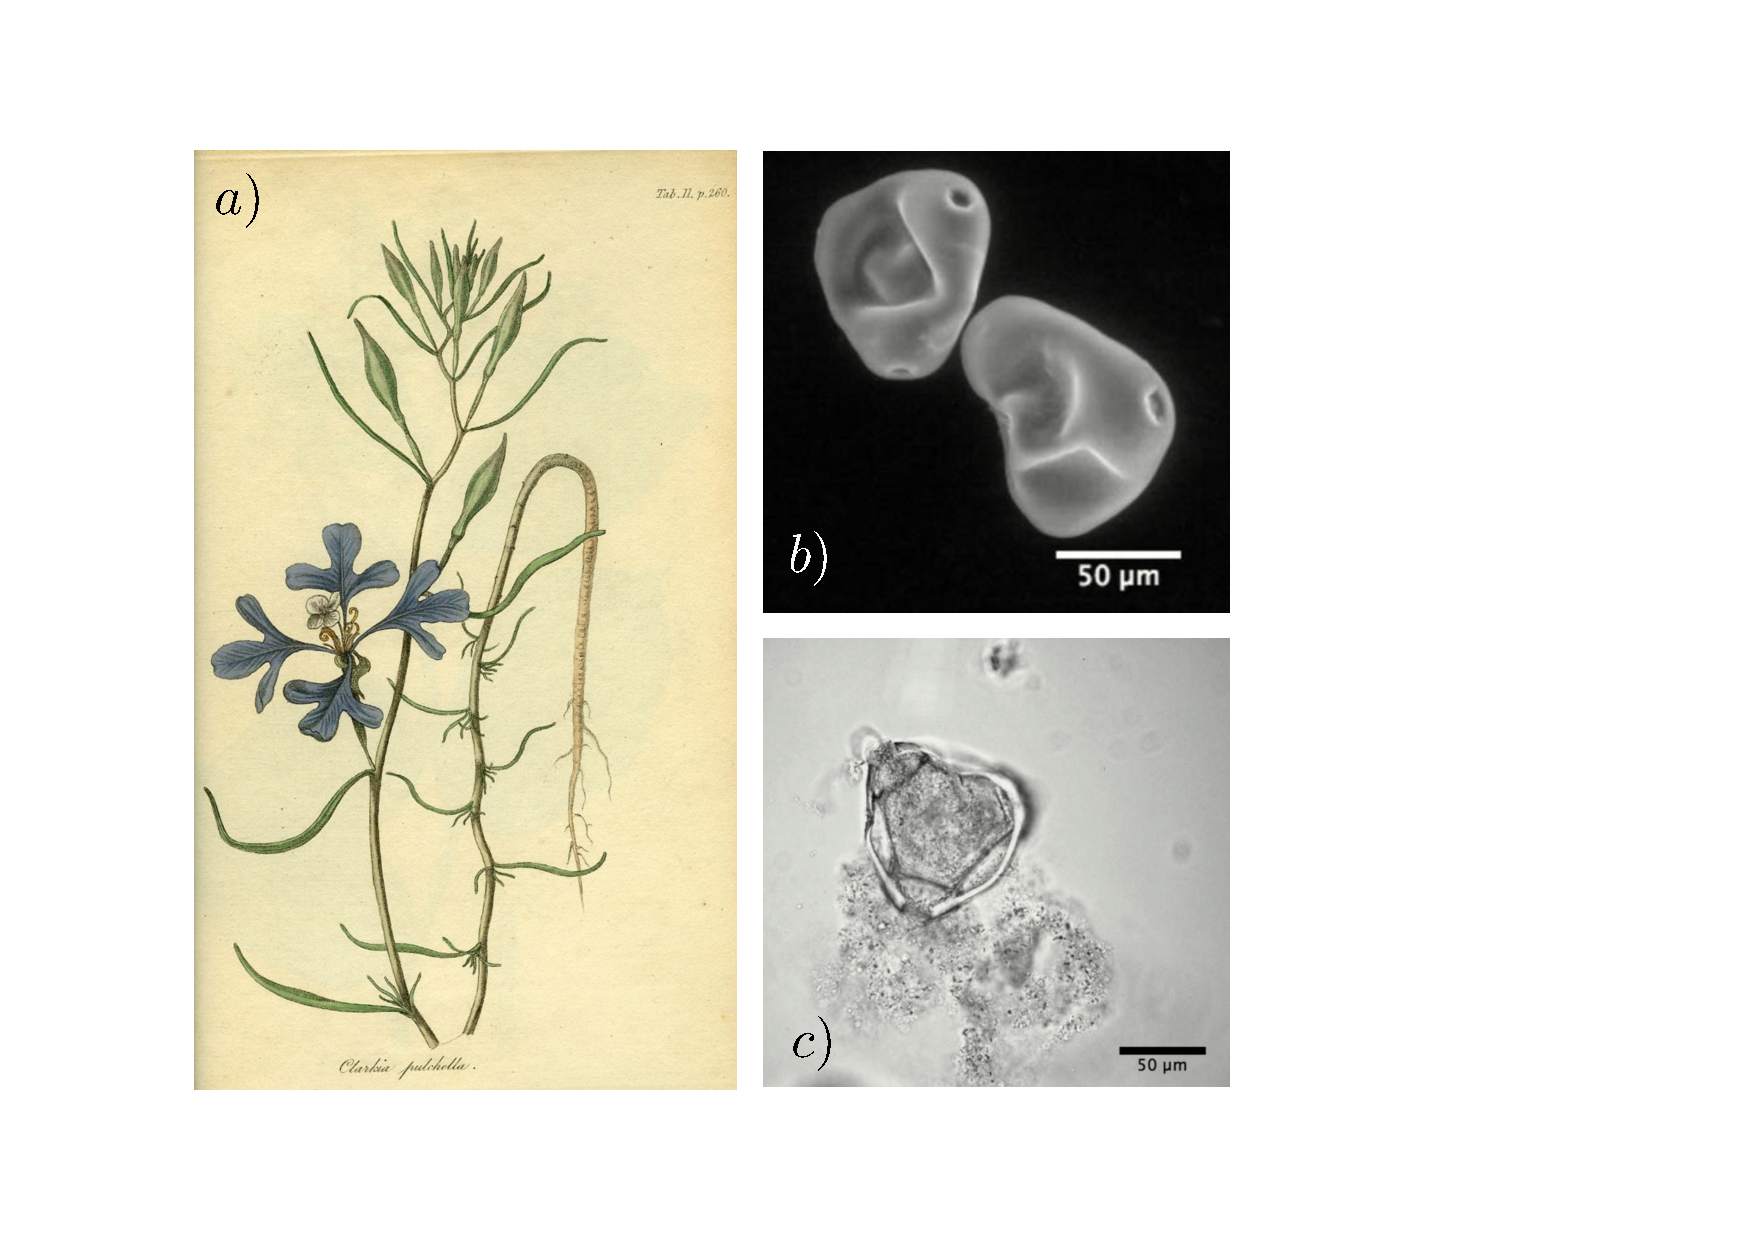
\includegraphics[width=.8\textwidth]{figures/chapter1/clarkia.pdf}
    \caption[\emph{Clarkia pulchella} and its pollen grains.]{\emph{Clarkia pulchella} and its pollen grains. $a)$ Painting of a \emph{Clarkia pulchella} specimen's anatomy by Frederick Pursh. $b)$ \emph{Clarkia} pollen grain under a microscope. $c)$ Bursting grain of pollen. $b)$ and $c)$ adapted from~\cite{pearle_brown_2010}.}
\end{figure}


Brown then repeated the experiment with other essences, and other parts of the specimens he was working on. The dance was still present, although from different sources than the male organelle. He concluded that if the process was alive, it was therefore not related to reproduction; pollen grains were not consciously seeking a mate through their motion. The then-widespread theory of George-Louis Leclerc that living things were built upon ``organic molecules'' seduced him; perhaps this motion could still owe to a living mechanism. The final blow to this theory of ``organic molecules'' with an intrinsic voluntary motion was dealt when he repeated the same observations with ``inert'' mineral dusts. 

This dance of ``molecules'', thought not formalised at the time, came to be known as \emph{``Brownian motion''}. 






\begin{figure}
     \centering
    \label{Perrin_rainbow}
    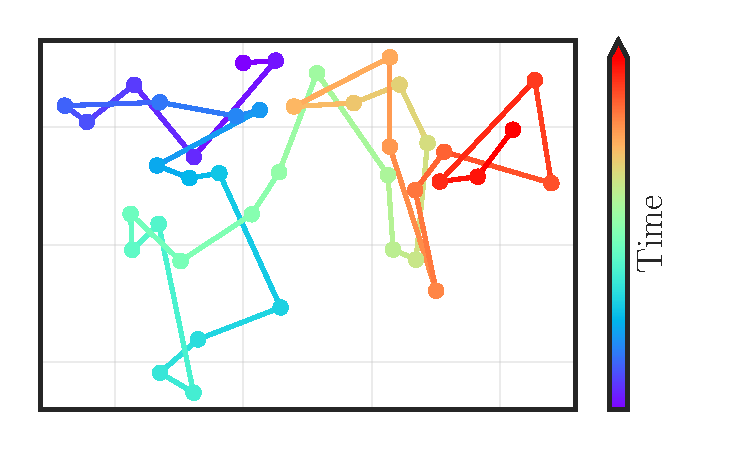
\includegraphics[width=1\textwidth]{figures/chapter1/Perrin_rainbow.pdf}
    \caption[Observation of the Brownian motion of a colloid in a fluid by Jean Perrin.]{Observation of the random and erratic motion of a colloid in a fluid by Jean Perrin (adapted from ``Mouvement brownien et réalité moléculaire'', 1909).}
\end{figure}



\section{Theoretical developments}
\subsection{The Fokker-Plank equation}

\begin{equation}
\mathrm{d}X_t = u(X_t)\mathrm{d}t + g \mathrm{d}B_t~,
\label{Fokker-Plank}
\end{equation}

where $u(X_t)$ is the drift velocity term, $g$ is the magnitude of the noise, and $\mathrm{d}B_t$ is the increment of a Wiener process.

We now take the average value of a function obeying the PDF $P(X_t, X_0; t)$, which we will call $f(X_t)$. This average value will, by definition, follow~\cite{LeBellac_2004}:

\begin{equation}
\langle f(X_t) \rangle = \int f(X_t) P(X_t, X_0; t) \mathrm{d}X_t~,
\label{avg_f}
\end{equation}

with the initial condition $P(X_t, X_0; 0) = \delta(X_t - X_0)$, where $\delta$ is the Dirac delta function. Expanding $f(X_t)$ in a Taylor series yields:

\begin{equation}
    f(X_t + \mathrm{d}X_t) = f(X_t) + f'(X_t) \mathrm{d}X_t + \frac{1}{2} f''(X_t) (\mathrm{d}X_t)^2 + \ldots
    \label{f_expansion}
\end{equation}

Substituting $\mathrm{d}X_t$ from the Fokker-Plank equation and taking the average, we get:

\begin{equation}
    \left\langle \frac{\mathrm{d}f(X_t)}{\mathrm{d}t} \right\rangle \simeq  \frac{\partial f(X_t)}{\partial X_t} u(X_t) + \frac{1}{2}  \frac{\partial^2 f(X_t)}{\partial X_t^2} g^2
    \label{f_avg_evolution}
\end{equation}

Combining this with the definition of the average value of $f(X_t)$, we can derive the Fokker-Plank equation for the PDF $P(X_t, X_0; t)$:
\begin{eqnarray}
\int \mathrm{d}X_t \frac{\partial f(X_t)}{\partial t} f(X_t) = \frac{\partial f(X_t)}{\partial X_t} u(X_t) + \frac{1}{2}  \frac{\partial^2 f(X_t)}{\partial X_t^2} g^2\\
= \int \mathrm{d}X_t\, P(X_t, X_0; t) G f(X_t)~,
\end{eqnarray}

where $G$ is the Generator, defined as $G = u(X_t) \frac{\partial}{\partial X_t} + \frac{1}{2} g^2 \frac{\partial^2}{\partial X_t^2}~$. Taking the adjoint of $G$ as $G^\dagger$, we can rewrite the above equation as:
\begin{equation}
    \int \mathrm{d}X_t\, P(X_t, X_0; t) G f(X_t) = \int \mathrm{d}X_t\, f(X_t) G^\dagger P(X_t, X_0; t)~.
\end{equation}

We can then derive the Fokker-Plank equation for the PDF $P(X_t, X_0; t)$ as:
\begin{equation}
    \frac{\partial P(X_t, X_0; t)}{\partial t} = G^\dagger P(X_t, X_0; t) = -\frac{\partial}{\partial X_t} \left( u(X_t) P(X_t, X_0; t) \right) + \frac{1}{2} \frac{\partial^2}{\partial X_t^2} \left( g^2 P(X_t, X_0; t) \right)~.
\end{equation}

Thus, for a bulk Brownian motion with Langevin equation
\begin{equation}
    \frac{\mathrm{d}x}{\mathrm{d}t} = \sqrt{2D_0} \eta(t)~,
    \label{Langevin_Fokker_plank_bulk}
\end{equation}

with $x$ the colloid's position, $D_0$ the bulk diffusion coefficient, and $\eta(t)$ a white noise of zero mean and unit variance, we can identify $u(x) = 0$ and $g = \sqrt{2D_0}$, and thus, the Fokker-Plank equation for the PDF of the colloid's position reads:
\begin{equation}
    \frac{\partial P(x, x_0; t)}{\partial t} = D_0 \frac{\partial^2 P(x, x_0; t)}{\partial x^2}~,
    \label{Fokker_Plank_bulk_diffusion_equation}
\end{equation}
which is the well-known diffusion equation.

\section{Advances and state of the Art}


\section{Bases of numerical simulations}